\documentclass[11pt, a4paper]{article}

% --- PACKAGES ---
\usepackage{tikz}
\usetikzlibrary{positioning, arrows.meta, shapes, backgrounds, fit, decorations.pathreplacing, calc}
\usepackage[utf8]{inputenc}
\usepackage[T1]{fontenc}
\usepackage[english]{babel}
\usepackage{geometry}
\geometry{top=2.5cm, bottom=2.5cm, left=2.5cm, right=2.5cm}
\usepackage{times}
\usepackage{graphicx}
\usepackage{wrapfig}
\usepackage{booktabs}
\usepackage{amsmath, amssymb, amsfonts}
\usepackage{hyperref}
\usepackage{float}
\usepackage{caption}
\usepackage{subcaption}
\usepackage{titlesec}
\usepackage{fancyhdr}
\usepackage{pdfpages} 
\usepackage{csquotes}
\usepackage{pgfgantt}
\usepackage{textcomp} % For the Euro symbol (€)

% --- FIX FOR WARNING ---
\setlength{\headheight}{14pt}

% --- BIBLIOGRAPHY SETUP ---
\usepackage[backend=biber, style=ieee]{biblatex}
\begin{filecontents}{references.bib}
@article{nie2025llada,
  title={Large Language Diffusion Models (LLaDA): A New Paradigm for Parallel Generation},
  author={Nie, Shuming and Zhang, Dan and Liu, X.},
  journal={arXiv preprint arXiv:2502.09992},
  year={2025}
}
@article{salimans2022progressive,
  title={Progressive Distillation for Fast Sampling of Diffusion Models},
  author={Salimans, Tim and Ho, Jonathan},
  journal={ICLR},
  year={2022}
}
@article{song2023consistency,
  title={Consistency Models},
  author={Song, Yang and Dhariwal, Prafulla},
  journal={ICML},
  year={2023}
}
@inproceedings{sahoo2024mdlm,
  title={Masked Diffusion Language Models},
  author={Sahoo, S. and Others},
  booktitle={NeurIPS},
  year={2024}
}
@article{vaswani2017attention,
  title={Attention is all you need},
  author={Vaswani, Ashish and others},
  journal={Advances in neural information processing systems},
  volume={30},
  year={2017}
}
@article{survey2025diffusion,
  title={A Comprehensive Survey on Diffusion Language Models: 2024-2026},
  author={Zhang, D. and Li, Y.},
  journal={IEEE Transactions on Pattern Analysis and Machine Intelligence},
  year={2026}
}
@techreport{strubell2019energy,
  title={Energy and Policy Considerations for Deep Learning in NLP},
  author={Strubell, Emma and Ganesh, Ananya and McCallum, Andrew},
  institution={University of Massachusetts Amherst},
  year={2019}
}
\end{filecontents}
\addbibresource{references.bib}

% --- HEADER/FOOTER ---
\pagestyle{fancy}
\fancyhf{}
\rhead{\textbf{GEP - Final Document}}
\lhead{Bachelor's Thesis (TFG)}
\rfoot{Page \thepage}

% --- DOCUMENT START ---
\begin{document}

% --- TITLE PAGE ---
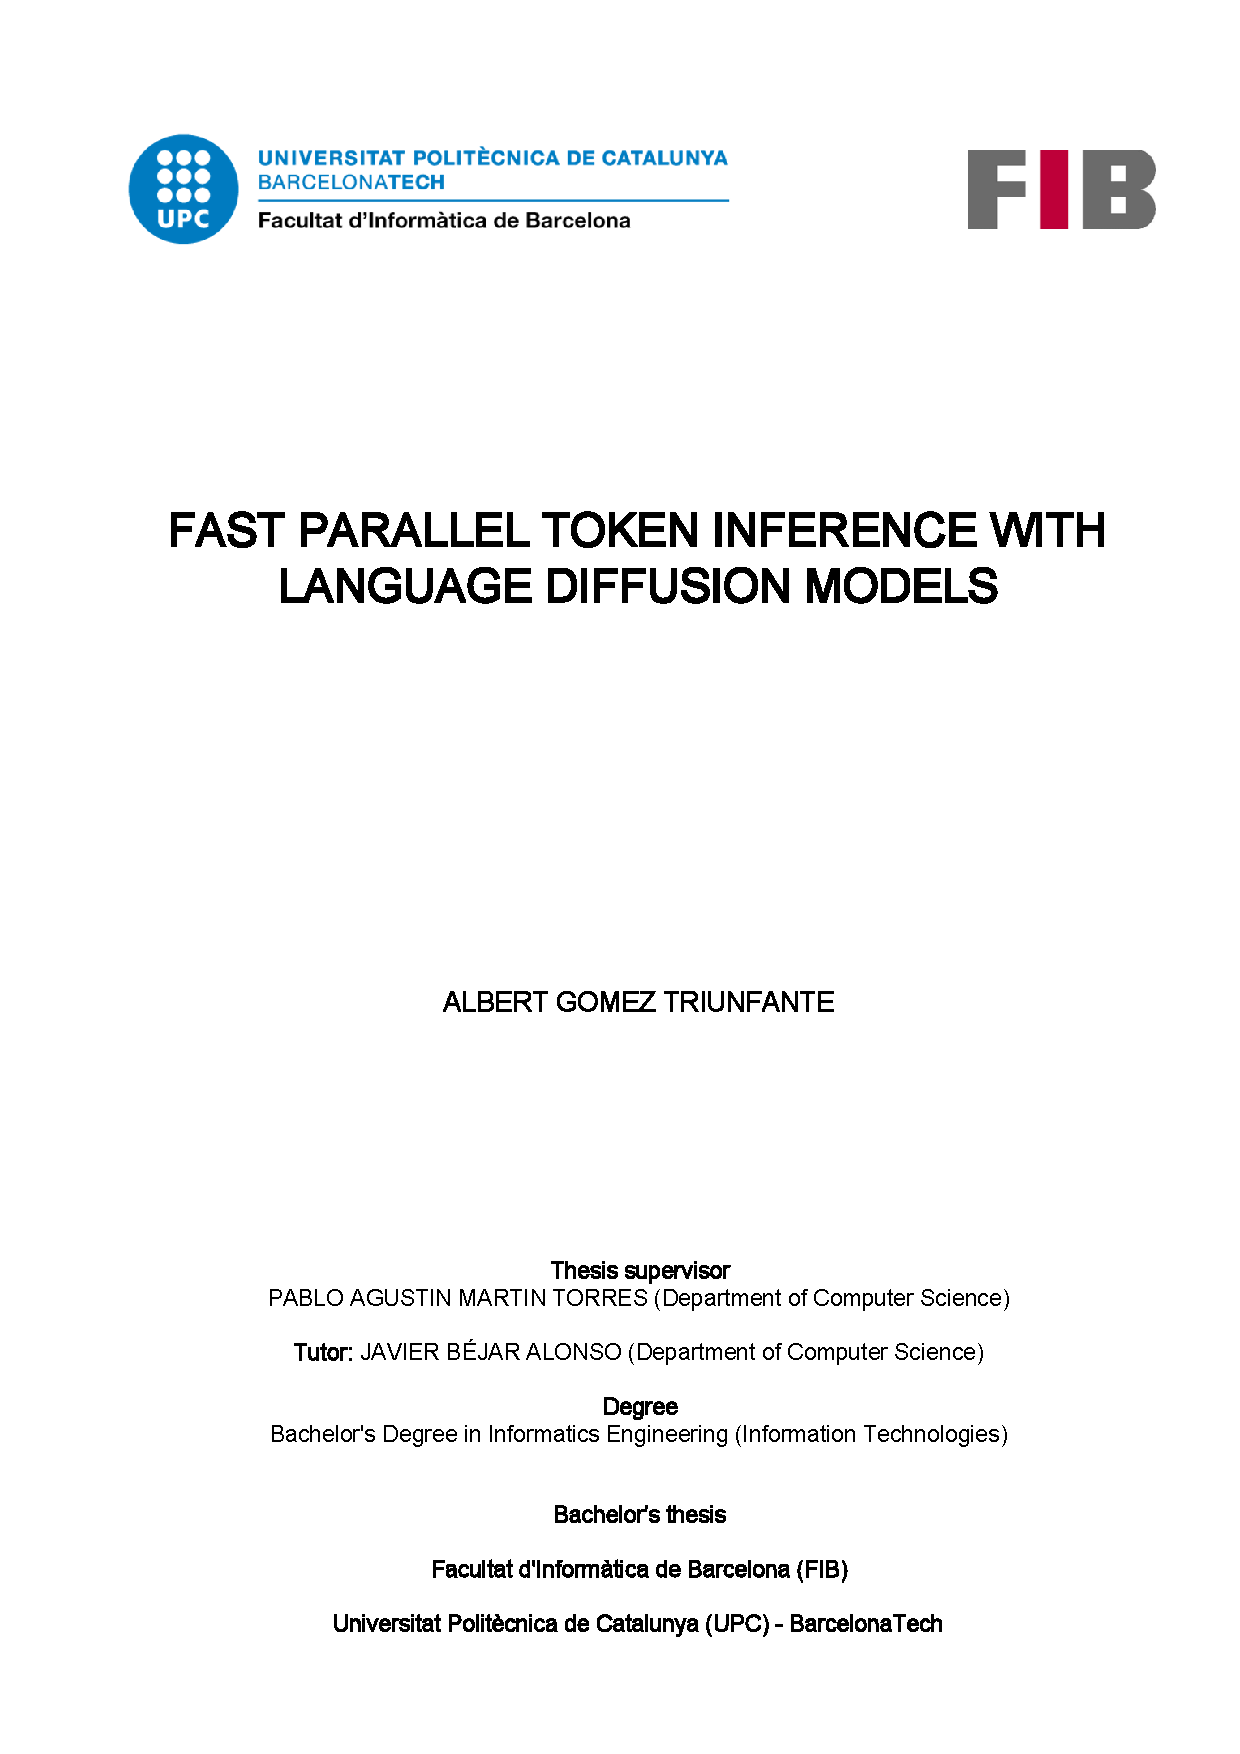
\includepdf[pages=-]{cover.pdf} 

\tableofcontents
\newpage

% ======================================================================
\section{Introduction and contextualization}
\label{sec:intro_context}

The field of Natural Language Processing (NLP) is currently dominated by Auto-Regressive (AR) Transformers (e.g., GPT-4, LLaMA), which generate text sequentially. While effective, this paradigm suffers from a linear latency bottleneck: generating $N$ tokens requires $N$ forward passes, leading to slow inference and suboptimal GPU utilization.

\textbf{Language Diffusion Models (LDMs)} \cite{nie2025llada} have emerged as a parallel alternative, theoretically capable of generating entire sequences simultaneously via iterative denoising. However, current LDMs still require a high number of sampling steps (typically 50--100) to reach convergence, which often negates their speed advantage over AR models.

In the domain of Computer Vision (Image Generation), this limitation was overcome by techniques such as \textbf{Progressive Distillation} \cite{salimans2022progressive} or Consistency Models \cite{song2023consistency}, where a "Student" model is trained to compress the "Teacher's" many denoising steps into a single or very few steps.

\textbf{Problem Statement:} While distillation techniques have revolutionized image generation, they have not yet been successfully adapted to the discrete and non-continuous domain of text diffusion.

\textbf{Thesis Proposal \& Institutional Context:} Within the specialization of \textbf{Information Technology (IT)} at the Facultat d'Informàtica de Barcelona (FIB), this project aims to implement and validate a \textbf{Knowledge Distillation} technique for Language Diffusion Models. By training a student LDM to mimic the trajectory of a pre-trained teacher LDM, we aim to achieve high-quality text generation in extremely few steps ($<10$), thereby unlocking the true potential of parallel token inference. Because deploying large-scale language models currently faces severe practical and economic constraints, this project is directly anchored in core IT themes: by drastically reducing the required denoising steps, we aim to maximize inference efficiency and significantly increase system throughput in production environments.

\subsection{The Auto-Regressive vs. Diffusion Paradigm}
Standard AR models estimate $P(x) = \prod P(x_t | x_{<t})$. This serial dependency prevents parallelization. LDMs, conversely, model the data distribution $p(x_0)$ by reversing a noise process $q(x_t | x_{t-1})$.
\begin{equation}
    x_{t-1} \leftarrow \text{Denoise}(x_t, \theta)
\end{equation}
While LDMs can predict all tokens in parallel, the iterative refinement requires $K$ steps. If $K$ is large, the latency advantage vanishes.

\begin{figure}[H]
    \centering
    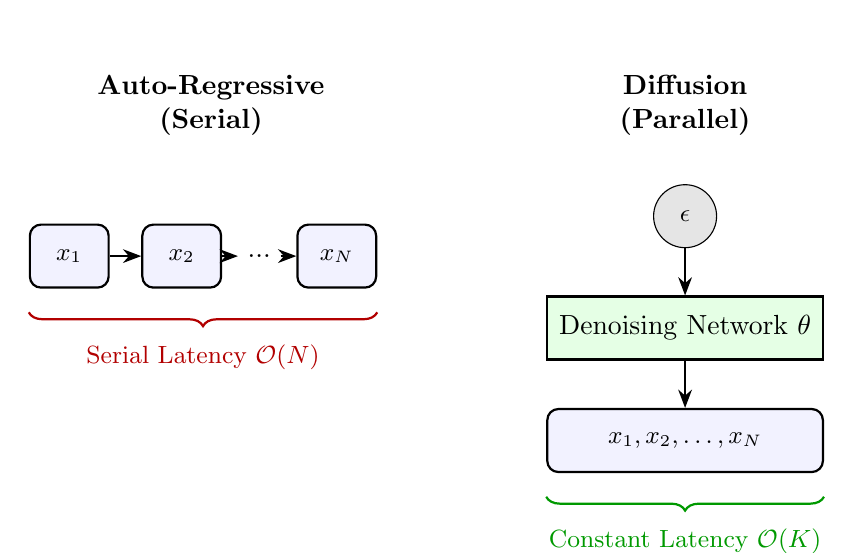
\begin{tikzpicture}[
        node distance=0.6cm and 0.8cm, 
        box/.style={draw, rectangle, rounded corners, minimum width=1.0cm, minimum height=0.8cm, align=center, fill=blue!5, thick, font=\small},
        noise/.style={draw, circle, fill=gray!20, minimum size=0.8cm, font=\small},
        arrow/.style={-Stealth, thick},
        title/.style={font=\bfseries, align=center}
    ]
    % --- LEFT: Auto-Regressive ---
    \node[title] (ar_title) {Auto-Regressive\\(Serial)};
    \node[box, below=1cm of ar_title, xshift=-1.8cm] (t1) {$x_1$};
    \node[box, right=0.4cm of t1] (t2) {$x_2$};
    \node[right=0.2cm of t2] (dots) {...};
    \node[box, right=0.2cm of dots] (tn) {$x_N$};
    \draw[arrow] (t1) -- (t2);
    \draw[arrow] (t2) -- (dots);
    \draw[arrow] (dots) -- (tn);
    \draw[decorate, decoration={brace, amplitude=5pt, mirror}, thick, red!70!black] 
        ([yshift=-0.3cm]t1.south west) -- ([yshift=-0.3cm]tn.south east) 
        node[midway, below=8pt, font=\small\color{red!70!black}] {Serial Latency $\mathcal{O}(N)$};

    % --- RIGHT: Diffusion ---
    \node[title, right=3.5cm of ar_title] (diff_title) {Diffusion\\(Parallel)};
    \node[noise, below=0.5cm of diff_title] (noise) {$\epsilon$};
    \node[draw, rectangle, fill=green!10, minimum width=3.5cm, minimum height=0.8cm, below=0.6cm of noise, thick] (denoise) {Denoising Network $\theta$};
    \node[box, below=0.6cm of denoise, minimum width=3.5cm] (output) {$x_1, x_2, \dots, x_N$};
    \draw[arrow] (noise) -- (denoise);
    \draw[arrow] (denoise) -- (output);
    \draw[decorate, decoration={brace, amplitude=5pt, mirror}, thick, green!60!black] 
        ([yshift=-0.3cm]output.south west) -- ([yshift=-0.3cm]output.south east) 
        node[midway, below=8pt, font=\small\color{green!60!black}] {Constant Latency $\mathcal{O}(K)$};
    \end{tikzpicture}
    \caption{Latency Comparison. \textbf{Left:} AR models generate tokens sequentially. \textbf{Right:} Diffusion models generate the entire sequence in parallel. \textit{Source: Compiled by the author.}}
    \label{fig:latency_comparison}
\end{figure}

\subsection{Current Limitations and Challenges in Discrete Diffusion}
While models like GPT-4 have set the standard for quality, their serial nature poses a fundamental limit on latency scaling. The time complexity of generating a sequence of length $N$ is $\mathcal{O}(N)$. As context windows grow to 128k or 1M tokens, this serial dependency becomes a bottleneck that no amount of parallel compute can solve purely through hardware scaling. Techniques like \textit{Speculative Decoding} attempt to mitigate this by drafting multiple tokens at once, but they are probabilistic and their speedup is upper-bounded (typically $2\times - 3\times$). Diffusion models, by contrast, offer a theoretical $\mathcal{O}(1)$ or $\mathcal{O}(K)$ complexity where $K$ is the number of denoising steps, independent of sequence length $N$.

As of early 2026, research on LDMs (e.g., LLaDA, MDLM) focuses on architecture and pre-training \cite{survey2025diffusion}. \textbf{There is a significant gap in post-training acceleration.} No open-source study has comprehensively applied progressive distillation to discrete text tokens, likely due to the difficulty of optimizing gradients over discrete categorical variables. This introduces significant challenges:
\begin{itemize}
    \item \textbf{Gradient Estimation:} We cannot backpropagate through discrete sampling operations (argmax). We must use the \textit{Concrete Distribution} (Gumbel-Softmax) or straight-through estimators to approximate gradients.
    \item \textbf{Rounding Errors:} In text, a slight error in the embedding space can flip a token from "happy" to "sad," destroying semantic coherence.
    \item \textbf{Loss Mismatch:} The standard Mean Squared Error (MSE) loss used in image distillation does not align well with the Cross-Entropy loss required for language modeling.
\end{itemize}

\subsection{Stakeholders}
\label{sec:stakeholders}
\begin{table}[H]
\centering
\caption{Stakeholder Analysis Matrix}
\label{tab:stakeholders}
\begin{tabular}{@{}lp{4cm}p{4cm}@{}}
\toprule
\textbf{Stakeholder} & \textbf{Interest (Motivation)} & \textbf{Power (Influence)} \\ \midrule
\textbf{Project Director} & High (Academic success, publication) & High (Approves scope/grade) \\
\textbf{The Student} & High (Learning, Career portfolio) & High (Executor) \\
\textbf{Scientific Community} & High (Reproducibility of new method) & Low (Passive observer) \\
\textbf{Industry (SMEs)} & Medium (Cost reduction in API) & Low (Potential future adopters) \\ \bottomrule
\end{tabular}
\end{table}

\textbf{Detailed Analysis:}
\begin{itemize}
    \item \textbf{Project Director:} Their primary concern is the feasibility of the scope. By strictly defining the boundaries (no pre-training, only distillation), we mitigate the risk of scope creep, ensuring the project is "finishable" within the TFG timeline.
    \item \textbf{The Student:} This project serves as a portfolio piece demonstrating mastery of advanced Deep Learning concepts (Diffusion, Distillation, PyTorch) that are highly sought after in top-tier AI research labs and tech companies.
    \item \textbf{Scientific Community:} If successful, the open-source code release will allow other researchers to replicate our distillation pipeline, potentially sparking a new wave of "Fast Text Diffusion" research.
\end{itemize}

\noindent \textbf{Strategy:} We will manage the \textit{Director} closely via bi-weekly meetings to align on the "Distillation Loss" formulation, while keeping the \textit{Scientific Community} in mind by ensuring the code is modular and open-source compatible.

% ======================================================================
\section{Justification of the chosen resolution alternative}
\label{sec:justification}

\subsection{Methodological Choice: Progressive Distillation vs. Alternatives}
When seeking to accelerate diffusion models, two primary strategies emerge: Consistency Models \cite{song2023consistency} and Progressive Distillation \cite{salimans2022progressive}. While Consistency Models map any point on the diffusion trajectory directly to the origin in a single step, they are notoriously difficult to adapt to discrete categorical domains like text. They rely on enforcing boundary conditions over continuous Ordinary Differential Equations (ODEs). 

In contrast, \textbf{Progressive Distillation} teaches a student model to take larger, discrete jump steps (e.g., matching 2 teacher steps in 1 student step). This discrete nature makes it significantly more adaptable to the token-by-token embedding space of language models. Therefore, this technique was selected as the most viable path to bridge the gap shown in Table \ref{tab:sota_comparison}.

\begin{table}[H]
\centering
\caption{Comparison of Generation Paradigms and the Thesis Gap}
\label{tab:sota_comparison}
\resizebox{\textwidth}{!}{%
\begin{tabular}{@{}lccccc@{}}
\toprule
\textbf{Paradigm} & \textbf{Example Model} & \textbf{Generation} & \textbf{Steps (N)} & \textbf{Latency} & \textbf{Quality} \\ \midrule
Auto-Regressive & GPT-4, LLaMA-3 & Serial & $N = \text{Length}$ & High (Linear) & SOTA \\
Standard Diffusion & SSD-LM, LLaDA & Parallel & $50 - 100$ & Med-High & High \\
Continuous Distillation & Stable Diffusion XL & Parallel & $4 - 8$ & Low & High \\
\textbf{Discrete Distillation} & \textbf{(This Thesis)} & \textbf{Parallel} & \textbf{4 - 8} & \textbf{Very Low} & \textbf{Target: High} \\ \bottomrule
\end{tabular}%
}
\end{table}

\subsection{Scientific Innovation}
Unlike a standard engineering project that benchmarks existing tools, this thesis proposes a \textbf{novel adaptation of an algorithm}. If successful, it contributes a new method to the NLP community: "Textual Progressive Distillation."

\subsection{Efficiency and Green AI}
Reducing the number of inference steps linearly reduces the energy required to generate text. If we reduce steps from 64 to 8, we reduce the energy cost by approximately $8\times$. This aligns with the "Green AI" initiative \cite{strubell2019energy} to make Large Language Models sustainable.

\subsection{Commercial Viability}
For real-time applications (e.g., conversational AI), latency is the primary KPI. A parallel model running in 4-8 steps could theoretically outperform LLaMA-3 by $5\times$--$10\times$ in wall-clock speed, making it highly valuable for industry. Consider a customer support chatbot that needs to generate a 200-token response:
\begin{itemize}
    \item \textbf{AR Model (LLaMA-3):} At 50 tokens/sec, this takes 4 seconds. This latency is noticeable and degrades user experience.
    \item \textbf{Standard LDM:} At 100 steps, it might also take 4 seconds or more.
    \item \textbf{Distilled LDM (Our Proposal):} With 4 steps, even if each step is heavier, the total latency could drop to 0.4 seconds.
\end{itemize}
This order-of-magnitude improvement ($10\times$) transforms the user experience from "waiting" to "instant," enabling new applications like real-time voice-to-voice translation where latency must be sub-500ms.

\subsection{Economic Impact}
Current LLM inference is prohibitively expensive. Companies like OpenAI and Anthropic spend millions daily on compute. A reduction in inference steps from 50 to 5 represents a potential $10\times$ reduction in GPU compute time per query. For an SME deploying a custom LDM, this technique could be the difference between a viable product and a bankrupt one.

% ======================================================================
\section{Scope of the project}
\label{sec:scope}

\subsection{General and Specific Objectives (SMART)}
The general objective is to implement and evaluate a \textbf{knowledge distillation technique} for Language Diffusion Models, training a "Student" model to compress the inference steps of a "Teacher" model, thereby achieving fast parallel text generation.
\begin{itemize}
    \item \textbf{O1 (Theoretical Framework):} Analyze the mathematical formulation of Progressive Distillation (Images) and adapt the loss function for discrete text data (Categorical Cross-Entropy / KL Divergence) by \textbf{March 15, 2026}.
    \item \textbf{O2 (Implementation):} Develop a "Teacher-Student" training loop in PyTorch, capable of loading a pre-trained LDM (e.g., MDLM/LLaDA) and fine-tuning the student weights, by \textbf{April 1, 2026}.
    \item \textbf{O3 (Distillation Training):} Train the student model on a subset of the OpenWebText dataset to reduce sampling steps from $N=64$ to $N=\{8, 4\}$, utilizing university or cloud GPU resources.
    \item \textbf{O4 (Validation):} Benchmark the "Distilled LDM" against the "Teacher LDM" and an "AR Baseline" (LLaMA-3), measuring \textbf{Speedup (x)} vs. \textbf{Quality Drop (Perplexity/BLEU)} by \textbf{May 20, 2026}.
\end{itemize}

\subsection{In-Scope vs. Out-of-Scope}
\textbf{In-Scope:} 
\begin{itemize}
    \item \textbf{Algorithm Adaptation:} Porting the distillation logic (step halving) from the continuous domain to the discrete text domain.
    \item \textbf{Model Distillation (Fine-tuning):} We assume the existence of a pre-trained "Teacher". We will not pre-train a model from scratch; we will only perform the distillation (fine-tuning) phase.
    \item \textbf{Target Models:} Open-source LDMs in the 1B-8B parameter range (e.g., MDLM, SSD-LM, LLaDA).
    \item \textbf{Evaluation:} Comparing the distilled model against the teacher on standard metrics (PPL, BLEU) and efficiency metrics (Latency, FLOPs).
\end{itemize}

\textbf{Out-of-Scope:} 
\begin{itemize}
    \item \textbf{Pre-training from Scratch:} We will not train the base LDM. We rely on published weights.
    \item \textbf{Novel Architectures:} We are not inventing a new Neural Network architecture (e.g., new Attention mechanism), but rather a new \textit{training method} for existing architectures.
    \item \textbf{Production Deployment:} The output is a scientific proof-of-concept, not a production API.
\end{itemize}

\subsection{Functional and Non-Functional Requirements}
\subsubsection{Functional Requirements}
\begin{itemize}
    \item The system must accept a text prompt as input and generate a coherent text continuation.
    \item The distillation pipeline must be able to load a pre-trained Teacher model and initialize a Student model with identical weights.
    \item The training loop must implement a specific loss function that handles discrete categorical data (e.g., Cross-Entropy with Soft-Targeting).
\end{itemize}

\subsubsection{Non-Functional Requirements}
\begin{itemize}
    \item \textbf{Performance:} The distilled model must achieve a latency reduction of at least $4\times$ compared to the teacher.
    \item \textbf{Quality:} The Perplexity (PPL) degradation of the student model must not exceed 15\% relative to the teacher.
    \item \textbf{Resources:} The fine-tuning process must fit within a single NVIDIA A100 (40GB/80GB) GPU using LoRA optimization.
\end{itemize}

\subsection{Validation Strategy and Metrics}
To ensure the scientific validity of our results, we will employ a rigorous evaluation protocol:
\begin{enumerate}
    \item \textbf{Teacher-Student Gap:} We will measure the KL-divergence between the teacher's output distribution and the student's. A low divergence indicates successful distillation.
    \item \textbf{Human Evaluation (Proxy):} We will use a strong LLM (e.g., GPT-4-Turbo) as a judge to rate the coherence of the distilled text compared to the teacher's text, identifying potential "hallucinations" introduced by the step reduction.
    \item \textbf{A/B Testing:} We will run side-by-side comparisons of latency on different batch sizes ($B=1, B=32$) to determine if the speedup holds under high-load production scenarios.
\end{enumerate}

% ======================================================================
\section{Time planning}
\label{sec:planning}

\subsection{Global Project Parameters and Methodology}
This project is formulated as a standard Bachelor's Thesis (TFG) for the Facultat d'Informàtica de Barcelona (FIB), corresponding to 18 ECTS credits. Therefore, the total workload is strictly planned for \textbf{540 hours}. It spans from February 10, 2026, to the expected defense on June 25, 2026 ($\sim 136$ days), requiring approx. 27.5 hours/week. 

This project adopts an \textbf{Agile Experimental Methodology}, adapted for research. Unlike a linear Waterfall approach, research requires iterative refinement of hypotheses. We divide the project into 2-week "Sprints." At the end of each sprint, a Sprint Review will be held with the Project Director to assess the achieved milestones, followed by a Sprint Retrospective to adjust the planning for the subsequent sprint based on empirical results.

\subsection{Work Breakdown Structure (WBS)}
To ensure granular tracking and mitigate risks, no single task in this planning exceeds the \textbf{50-hour maximum threshold} mandated by the GEP guidelines.

\textbf{Concurrent Tasks (Cross-cutting)}
These tasks span the entire duration of the project.
\begin{itemize}
    \item \textbf{PM1: GEP Course Deliverables [40h].} Involves drafting, formatting, and refining the Context, Planning, Budget, and Final GEP deliverables. The 40-hour estimate is justified as each of the 4 major documents requires approximately 10 hours of dedicated writing and formatting.
    \item \textbf{PM2: Weekly Sprint Planning \& Director Meetings [20h].} Involves preparing agendas and reviewing progress. The 20-hour estimate corresponds to one hour per week over the $\sim20$-week duration of the project.
    \item \textbf{DOC1: State of the Art drafting [25h].} Reading selected papers and synthesizing them into the academic framework. 25 hours is necessary due to the dense mathematical nature of recent diffusion models.
    \item \textbf{DOC2: Methodology \& Experiments drafting [35h].} Documenting the code architecture, loss functions, and experimental setups. This takes 35 hours because it runs continuously alongside Sprints 2, 3, and 4.
    \item \textbf{DOC3: Final memory review and formatting [20h].} Proofreading, LaTeX compilation fixes, and bibliography checks before final submission.
\end{itemize}

\textbf{Sprint Breakdown}
\begin{itemize}
    \item \textbf{Sprint 1: Theoretical Setup (Feb 10 - Mar 8) [80h]}
    \begin{itemize}
        \item \textbf{T1.1: Literature review on Discrete Diffusion [30h].} This task involves reading roughly 15 key papers to extract current methodologies. It requires 30 hours because adapting continuous image algorithms to discrete text requires a deep understanding of complex probability flows.
        \item \textbf{T1.2: Mathematical formulation of Loss Function [30h].} Deriving the exact equations to be coded later (e.g., KL-Divergence soft-targets). The 30-hour estimate is justified by the heavy mathematical adaptation required to bridge the gap between continuous MSE and categorical Cross-Entropy.
        \item \textbf{T1.3: Teacher model validation [20h].} Downloading the LLaDA weights and setting up a basic inference script to verify the open-source model works. 20 hours is assigned to handle potential undocumented environment dependencies.
    \end{itemize}

    \item \textbf{Sprint 2: Pipeline Implementation (Mar 9 - Apr 5) [90h]}
    \begin{itemize}
        \item \textbf{T2.1: Setup PyTorch environment [20h].} Configuring CUDA, HuggingFace libraries, and resolving dependency conflicts on the local PC.
        \item \textbf{T2.2: Implement DistillationTrainer class [35h].} Writing the core Python class that will handle the forward passes of both Teacher and Student models. This demands 35 hours because it requires overriding standard PyTorch training loops to implement custom backward passes and gradient approximations.
        \item \textbf{T2.3: WandB integration \& Toy Task [35h].} Integrating logging and verifying convergence on a tiny dataset (TinyShakespeare). This takes 35 hours as it acts as the primary debugging phase for the mathematical logic coded in T2.2.
    \end{itemize}

    \item \textbf{Sprint 3: Scale-up \& Initial Training (Apr 6 - May 3) [90h]}
    \begin{itemize}
        \item \textbf{T3.1: LoRA configuration for 8B model [30h].} Setting up Low-Rank Adaptation matrices to avoid VRAM overflow. 30 hours is justified as finding the optimal rank ($r$) and target modules requires several trial-and-error runs on the cloud GPU.
        \item \textbf{T3.2: Initial training run (N=16) \& gradient debugging [40h].} The actual distillation process. This is the most demanding task (40h) because discrete distillation is notoriously unstable; it requires active monitoring, pausing the run, and deploying immediate code patches to handle exploding gradients.
        \item \textbf{T3.3: Hyperparameter tuning [20h].} Adjusting the learning rate and soft-target weights based on T3.2 results to ensure smooth loss convergence.
    \end{itemize}

    \item \textbf{Sprint 4: Advanced Training \& Benchmarks (May 4 - May 31) [90h]}
    \begin{itemize}
        \item \textbf{T4.1: Final distillation runs (N=8, N=4 steps) [40h].} Executing the final training iterations to compress the model further. This requires 40 hours of passive monitoring and managing various model checkpoints over long cloud compute sessions.
        \item \textbf{T4.2: Inference latency profiling [20h].} Using CodeCarbon and precise timers to measure tokens/second and energy consumption compared to the Teacher model.
        \item \textbf{T4.3: Quality evaluation [30h].} Computing Perplexity (PPL) and BLEU scores on the Wikitext-103 dataset. 30 hours is needed because calculating valid PPL on large datasets requires generating millions of tokens, which is highly time-consuming even on accelerated hardware.
    \end{itemize}

    \item \textbf{Sprint 5: Wrap-up \& Defense (Jun 1 - Jun 25) [50h]}
    \begin{itemize}
        \item \textbf{T5.1: Final Results analysis and charting [20h].} Aggregating raw CSV data from T4.3 into professional academic plots using Matplotlib.
        \item \textbf{T5.2: Presentation slide deck creation [20h].} Condensing the 50-page thesis into a concise 15-minute visual presentation.
        \item \textbf{T5.3: Oral defense rehearsal [10h].} Practicing pacing and anticipating Q\&A with the Project Director.
    \end{itemize}
\end{itemize}

\subsection{Task Summary and Resources Table}
\begin{table}[H]
\centering
\caption{Detailed Task Summary mapped to Required Resources}
\label{tab:tasks}
\resizebox{\textwidth}{!}{%
\begin{tabular}{@{}llccl@{}}
\toprule
\textbf{Code} & \textbf{Descriptive Name} & \textbf{Hours} & \textbf{Dependencies} & \textbf{Specific Resources} \\ \midrule
PM1 & GEP Deliverables & 40 & None & Local PC, LaTeX, GEP Materials \\
PM2 & Sprint Meetings & 20 & None & Local PC, Google Meet, Director \\
DOC1 & State of the Art Draft & 25 & T1.1 & Local PC, Mendeley, IEEE Xplore \\
DOC2 & Methodology Draft & 35 & T3.2 & Local PC, LaTeX \\
DOC3 & Final Review & 20 & T4.3, T5.1 & Local PC, Grammarly \\ \midrule
T1.1 & Literature Review & 30 & None & Local PC, arXiv \\
T1.2 & Loss Formulation & 30 & T1.1 & Local PC, Overleaf \\
T1.3 & Teacher Validation & 20 & None & Local PC, HuggingFace \\ \midrule
T2.1 & Setup Environment & 20 & None & Local PC, Python, PyTorch \\
T2.2 & DistillationTrainer & 35 & T1.2, T2.1 & Local PC, GitHub \\
T2.3 & Toy Task & 35 & T2.2 & Local PC, WandB \\ \midrule
T3.1 & LoRA Configuration & 30 & T2.2 & A100 GPU (Cloud/Cluster) \\
T3.2 & Initial Training Run & 40 & T2.3, T3.1 & A100 GPU, WandB \\
T3.3 & Hyperparameter Tuning & 20 & T3.2 & A100 GPU \\ \midrule
T4.1 & Final Distillation Runs & 40 & T3.3 & A100 GPU, HuggingFace \\
T4.2 & Latency Profiling & 20 & T4.1 & Local PC / T4 GPU, CodeCarbon \\
T4.3 & Quality Evaluation & 30 & T4.1 & Local PC, BLEU/PPL Scripts \\ \midrule
T5.1 & Results Analysis & 20 & T4.2, T4.3 & Local PC, Matplotlib \\
T5.2 & Slide Deck Creation & 20 & T5.1 & Local PC, PowerPoint/Beamer \\
T5.3 & Defense Rehearsal & 10 & T5.2 & Local PC, Project Director \\ \bottomrule
\end{tabular}%
}
\end{table}

\subsection{Agile Gantt Chart}
\begin{figure}[H]
    \centering
    \begin{ganttchart}[
        vgrid={*4{draw=none}, *1{dotted}}, 
        hgrid,
        expand chart=\textwidth, 
        y unit title=0.45cm,
        y unit chart=0.35cm,
        bar/.append style={fill=blue!30, draw=blue!60}, 
        bar height=0.6,
        group right shift=0,
        group top shift=0.7,
        group height=.3,
        group/.append style={fill=black!80}
    ]{1}{20} 
    \gantttitle{Feb}{3} 
    \gantttitle{March}{4} 
    \gantttitle{April}{4} 
    \gantttitle{May}{5} 
    \gantttitle{June}{4} \\
    \gantttitlelist{1,...,20}{1} \\

    \ganttgroup{Concurrent (Agile)}{1}{20} \\
    \ganttbar{PM1 \& PM2}{1}{20} \\
    \ganttbar{DOC1, DOC2, DOC3}{2}{19} \\

    \ganttgroup{SP1: Theory \& Setup}{1}{4} \\
    \ganttbar[bar/.append style={fill=green!30}]{T1.1: Literature Review}{1}{2} \\
    \ganttbar[bar/.append style={fill=green!30}]{T1.2: Loss Formulation}{2}{3} \\
    \ganttbar[bar/.append style={fill=green!30}]{T1.3: Teacher Validation}{3}{4} \\

    \ganttgroup{SP2: Pipeline Dev}{5}{8} \\
    \ganttbar[bar/.append style={fill=green!30}]{T2.1: Setup Environment}{5}{5} \\
    \ganttbar[bar/.append style={fill=green!30}]{T2.2: DistillationTrainer}{6}{7} \\
    \ganttbar[bar/.append style={fill=green!30}]{T2.3: Toy Task}{7}{8} \\

    \ganttgroup{SP3: Initial Training}{9}{12} \\
    \ganttbar[bar/.append style={fill=orange!40}]{T3.1: LoRA Configuration}{9}{10} \\
    \ganttbar[bar/.append style={fill=orange!40}]{T3.2: Initial Training Run}{10}{11} \\
    \ganttbar[bar/.append style={fill=orange!40}]{T3.3: Hyperparameter Tuning}{12}{12} \\

    \ganttgroup{SP4: Final Runs \& Benchmarks}{13}{16} \\
    \ganttbar[bar/.append style={fill=orange!40}]{T4.1: Final Distillation Runs}{13}{14} \\
    \ganttbar[bar/.append style={fill=orange!40}]{T4.2: Latency Profiling}{15}{15} \\
    \ganttbar[bar/.append style={fill=orange!40}]{T4.3: Quality Evaluation}{15}{16} \\

    \ganttgroup{SP5: Wrap-up}{17}{19} \\
    \ganttbar[bar/.append style={fill=purple!30}]{T5.1: Results Analysis}{17}{17} \\
    \ganttbar[bar/.append style={fill=purple!30}]{T5.2: Slide Deck Creation}{18}{18} \\
    \ganttbar[bar/.append style={fill=purple!30}]{T5.3: Defense Rehearsal}{19}{19} \\
    
    \ganttmilestone{Thesis Defense}{20} 
    \end{ganttchart}
    \caption{Granular Agile Gantt Chart mapping sub-tasks 1:1 to the WBS. \textit{Source: Compiled by the author.}}
    \label{fig:detailed_gantt}
\end{figure}

\subsection{Risk Management \& Alternative Plans}
As required by project management standards, we have defined "Plan B" tasks for critical risks. These alternative tasks replace primary tasks if a risk materializes, ensuring the project \textbf{still finishes by June 25}.

\textbf{Risk 1: Severe VRAM Limitations (Hardware Failure).} If the NVIDIA A100 GPU becomes unavailable or if the 8B parameter model Cannot fit in memory even with LoRA (during Sprint 3).
\begin{itemize}
    \item \textbf{Plan B Task (ALT-T3.1):} Switch to a smaller Teacher model (e.g., a 1.5B or 3B diffusion model).
    \item \textbf{Time Impact \& Schedule Adjustment:} Requires an estimated 15 hours to download, integrate, and validate the new model. We will absorb these 15 hours by reducing the scope of \textbf{T4.3} (Quality Evaluation). Instead of running extensive benchmarks on multiple datasets, we will restrict evaluation to a single dataset (Wikitext-103). The final delivery date remains unchanged.
    \item \textbf{Additional Resources Required:} Access to the HuggingFace Model Hub to locate and download the alternative architecture. It will also require consulting the specific API documentation for the new model, though no additional human resources (staff) are needed.
\end{itemize}

\textbf{Risk 2: Distillation Training Instability.} If the Student model's loss diverges completely or suffers from mode collapse during \textbf{T3.2} (Sprint 3).
\begin{itemize}
    \item \textbf{Plan B Task (ALT-T3.2):} Abandon the KL-Divergence soft-target approach and revert to standard feature-matching loss (MSE on hidden states), which is vastly more stable but yields slightly worse text generation quality.
    \item \textbf{Time Impact \& Schedule Adjustment:} Requires 20 hours to rewrite the loss function in the \texttt{DistillationTrainer} and restart the run. To recover these 20 hours, \textbf{T4.1} (Final Distillation Runs) will be simplified. We will only distill to N=8 steps instead of testing both N=8 and N=4. The project successfully concludes on time with a slightly narrower scope.
    \item \textbf{Additional Resources Required:} This pivot will require an ad-hoc technical consultation (approx. 1-2 hours) with the Thesis Director to validate the new MSE approach. Additionally, because the failed run will have consumed initial budget, it requires re-allocating extra Cloud GPU (A100) time to execute the new training loop.
\end{itemize}


% ======================================================================
\section{Budget}
\label{sec:budget}

This section details the economic planning required to execute the thesis, adhering to the 540-hour workload defined in the project scope. Cost estimations include a standard 1.35 multiplier for Social Security contributions, referencing average gross salaries for Junior IT roles in Spain (Data: Glassdoor \& InfoJobs, 2025).

\subsection{Identification of Costs and Staff Estimates}
To guarantee full granularity, the 540 hours have been broken down by every individual sub-task defined in the Gantt chart. Each task is mapped to the exact hourly cost of the assigned professional role.

\begin{table}[H]
\centering
\caption{Highly Granular Staff Costs Broken Down by Individual Gantt Chart Task}
\label{tab:hr_budget}
\resizebox{\textwidth}{!}{%
\begin{tabular}{@{}llcccc@{}}
\toprule
\textbf{Task Code} & \textbf{Assigned Role} & \textbf{Hours} & \textbf{Gross Rate} & \textbf{Rate w/ SS (x1.35)} & \textbf{Total Cost (€)} \\ \midrule
PM1 & Project Manager & 40 & 25.00 €/h & 33.75 €/h & 1,350.00 \\
PM2 & Project Manager & 20 & 25.00 €/h & 33.75 €/h & 675.00 \\
DOC1 & AI Researcher & 25 & 20.00 €/h & 27.00 €/h & 675.00 \\
DOC2 & AI Researcher & 35 & 20.00 €/h & 27.00 €/h & 945.00 \\
DOC3 & AI Researcher & 20 & 20.00 €/h & 27.00 €/h & 540.00 \\
T1.1 & AI Researcher & 30 & 20.00 €/h & 27.00 €/h & 810.00 \\
T1.2 & AI Researcher & 30 & 20.00 €/h & 27.00 €/h & 810.00 \\
T1.3 & ML Engineer & 20 & 15.00 €/h & 20.25 €/h & 405.00 \\
T2.1 & ML Engineer & 20 & 15.00 €/h & 20.25 €/h & 405.00 \\
T2.2 & ML Engineer & 35 & 15.00 €/h & 20.25 €/h & 708.75 \\
T2.3 & ML Engineer & 35 & 15.00 €/h & 20.25 €/h & 708.75 \\
T3.1 & ML Engineer & 30 & 15.00 €/h & 20.25 €/h & 607.50 \\
T3.2 & ML Engineer & 40 & 15.00 €/h & 20.25 €/h & 810.00 \\
T3.3 & ML Engineer & 20 & 15.00 €/h & 20.25 €/h & 405.00 \\
T4.1 & ML Engineer & 40 & 15.00 €/h & 20.25 €/h & 810.00 \\
T4.2 & ML Engineer & 20 & 15.00 €/h & 20.25 €/h & 405.00 \\
T4.3 & AI Researcher & 30 & 20.00 €/h & 27.00 €/h & 810.00 \\
T5.1 & AI Researcher & 20 & 20.00 €/h & 27.00 €/h & 540.00 \\
T5.2 & Project Manager & 20 & 25.00 €/h & 33.75 €/h & 675.00 \\
T5.3 & Project Manager & 10 & 25.00 €/h & 33.75 €/h & 337.50 \\ \midrule
\textbf{Total Staff Cost} & & \textbf{540} & & & \textbf{13,432.50} \\ \bottomrule
\end{tabular}%
}
\end{table}

\subsection{General Costs and Amortization}
General costs include hardware, software, and operational expenses. Hardware amortization is calculated over a standard 4-year (1,460 days) useful life, prorated for the 4.5 months ($\approx 136$ days) of the project duration.
\begin{itemize}
    \item \textbf{Hardware (Local PC):} Valued at 1,500 €. Amortization: $1,500 \text{ €} \times (136 / 1460) = 139.72 \text{ €}$.
    \item \textbf{Hardware (Cloud GPU):} Rental of an NVIDIA A100 GPU for 100 hours of training at an estimated 2.50 €/h. This is a direct consumption cost: $250.00 \text{ €}$.
    \item \textbf{Software Licenses:} PyTorch, HuggingFace, and standard IDEs are open-source. GitHub Pro and Overleaf are covered via University Student Packs (0.00 €).
    \item \textbf{Operational Costs:} Electricity (540h $\times$ 0.5 kW $\times$ 0.20 €/kWh = 54.00 €) and workspace/internet overhead estimated at 150.00 €.
\end{itemize}
\textbf{Total General Costs:} \textbf{593.72 €}

\subsection{Contingencies and Incidentals}
To ensure financial robustness, indirect costs are calculated based on standard IT risk margins and the specific risk matrix defined previously.
\begin{itemize}
    \item \textbf{Contingency Margin:} A standard margin of \textbf{15\%} of the cumulative direct costs (Staff + General, totaling 14,026.22 €) is applied to cover unforeseen general project delays. This yields a contingency reserve of \textbf{2,103.93 €}.
    \item \textbf{Incidentals:} Calculated based on specific risks, weighted by their probability:
    \begin{itemize}
        \item \textit{Risk 1 (VRAM limitations):} 15 extra hours of ML Engineer time (303.75 €). Estimated probability: 30\%. Expected cost = 91.12 €.
        \item \textit{Risk 2 (Training Instability):} 20 extra hours of ML Engineer time (405.00 €). Estimated probability: 40\%. Expected cost = 162.00 €.
    \end{itemize}
\end{itemize}

\subsection{Total Budget Summary}
\begin{table}[H]
\centering
\caption{Total Project Budget Summary}
\label{tab:total_budget}
\begin{tabular}{@{}lr@{}}
\toprule
\textbf{Concept} & \textbf{Amount (€)} \\ \midrule
\textbf{Direct Costs} & \textbf{14,026.22} \\
\hspace{0.5cm} Human Resources & 13,432.50 \\
\hspace{0.5cm} General Costs & 593.72 \\ \midrule
\textbf{Indirect Costs} & \textbf{2,357.05} \\
\hspace{0.5cm} Contingency Margin (15\%) & 2,103.93 \\
\hspace{0.5cm} Incidentals (Risk-weighted) & 253.12 \\ \midrule
\textbf{Total Project Budget} & \textbf{16,383.27} \\ \bottomrule
\end{tabular}
\end{table}

\subsection{Management Control}
To effectively control potential budget deviations during execution, financial indicators will be monitored at the end of every Agile Sprint. If the Cost Performance Index ($CPI = EV/AC$) drops below 0.90 at any sprint review, non-critical validation tasks (e.g., extensive multi-dataset benchmarking) will be descoped to re-align the budget dynamically without requiring additional funding.

% ======================================================================
\section{Sustainability and social commitment}
\label{sec:sustainability}

\subsection{Self-Assessment Summary}
Prior to completing the sustainability questionnaire, my understanding of sustainability in software engineering was largely limited to superficial hardware power consumption. The self-assessment revealed a significant blind spot in my perspective: I had not fully considered the socioeconomic implications of democratizing Artificial Intelligence, nor the full lifecycle costs of training Large Language Models (LLMs). 

\textbf{Strengths:} A major strength identified during this assessment is my project's inherent alignment with "Green AI" principles; by focusing on Knowledge Distillation, the core objective is inherently sustainable (reducing inference compute). 

\textbf{Weaknesses:} However, a weakness identified is the lack of a formal carbon-tracking protocol during my own model's training phase. Moving forward, I am committed to integrating tools like \texttt{CodeCarbon} into my pipeline to measure the actual CO$_2$ emissions of the distillation process itself, ensuring that the environmental cost of the "Student" training does not outweigh the benefits gained during inference. This reflection has transformed my view of the TFG from a purely technical algorithm-optimization task into a holistic Information Technology solution designed to solve real-world energy and accessibility bottlenecks.

\subsection{Economic Dimension}
\begin{itemize}
    \item \textbf{Reflection on Estimated Cost:} The estimated project cost of $\approx$ 16,383 € is highly competitive when viewed as an R\&D investment. Developing a custom accelerated Language Diffusion Model (LDM) from scratch would cost exponentially more in human and compute resources.
    \item \textbf{State of the Art (Current Solutions):} Currently, deploying LLMs in production is prohibitively expensive. Inference for autoregressive models scales linearly with token length, requiring massive GPU clusters running 24/7, costing companies thousands of euros daily.
    \item \textbf{Improvement:} By reducing inference steps from $>50$ down to $<10$, this distillation technique drastically cuts the server time required per query. This reduces the economic barrier to entry, allowing SMEs to deploy sophisticated language models without needing premium, high-tier GPU infrastructure.
\end{itemize}

\subsection{Environmental Dimension}
\begin{itemize}
    \item \textbf{Project Impact \& Minimization:} Training the distilled model will consume significant GPU power (estimated 100 hours on an A100). To minimize this impact, the project avoids training from scratch, instead reusing pre-trained weights via LoRA, which reduces trainable parameters by 99\% and slashes training energy.
    \item \textbf{State of the Art (Current Solutions):} Standard AR models and non-distilled LDMs are environmentally taxing due to the massive energy draw (and subsequent cooling requirements) of data centers executing long, sequential generation passes.
    \item \textbf{Improvement:} This solution directly addresses the carbon footprint of AI inference. By requiring 80\% fewer computational steps to generate the same text, the energy consumed per query drops proportionally, directly contributing to a lower global carbon footprint for AI services.
\end{itemize}

\subsection{Social Dimension}
\begin{itemize}
    \item \textbf{Personal Growth:} This project forces me to master state-of-the-art Deep Learning concepts (Diffusion, PyTorch, Distillation) and bridge the gap between theoretical math and practical IT deployment, significantly enhancing my professional engineering profile.
    \item \textbf{State of the Art \& Real Need:} Currently, the power of cutting-edge AI is concentrated in the hands of a few tech giants who can afford the hardware. There is a real societal need to democratize this technology to prevent technological monopolies.
    \item \textbf{Improvement:} By optimizing models to run faster and on less expensive hardware, this project contributes to making advanced NLP tools accessible to independent researchers, educators, and underfunded institutions, thereby improving equity in the tech landscape.
\end{itemize}

\newpage
% ======================================================================
\printbibliography

\end{document}